\documentclass[11pt,a4paper]{article}
			\usepackage[french]{babel}
					
				\usepackage{pifont}  
				\usepackage[utf8x]{inputenc}
				\usepackage[T1]{fontenc} 
				\usepackage{lmodern}			
				\usepackage{fancyhdr}
				\usepackage{textcomp}
				\usepackage{makeidx}
				\usepackage{tabularx}
				\usepackage{multicol}
				\usepackage{multirow}
				\usepackage{longtable}
				\usepackage{color}
				\usepackage{soul}
				\usepackage{boxedminipage}
				\usepackage{shadow}
				\usepackage{framed}			
				\usepackage{array}
				\usepackage{url}
				\usepackage{ragged2e}
				\usepackage{fancybox}
				\newcommand{\cadretitre}[2]{
				  \vspace*{0.8\baselineskip}
				  \begin{center}%
				  \boxput*(0,1){%
					%\colorbox{white}{\Large\textbf{\ #1\ }}%
				  }%
				  {%
					\setlength{\fboxsep}{10pt}%
				    \Ovalbox{\begin{minipage}{.8\linewidth}\begin{center}\Large\sffamily{#2}\end{center}\end{minipage}}}%
				  \end{center}
				  \vspace*{2\baselineskip}
				  }
			
			\makeatletter
			\def\@seccntformat#1{\protect\makebox[0pt][r]{\csname the#1\endcsname\quad}}
			\makeatother

				% Permet d'afficher qqchose à une positin absolue
				\usepackage[absolute]{textpos}
				\setlength{\TPHorizModule}{1cm}
				\setlength{\TPVertModule}{\TPHorizModule}
	
				\usepackage[titles]{tocloft}
				\setlength{\cftbeforesecskip}{0.5ex}
				\setlength{\cftbeforesubsecskip}{0.2ex}
				\addto\captionsfrench{\renewcommand\contentsname{}}
				
				\usepackage[font=scriptsize]{caption}
				
				\usepackage{listings}
\lstdefinestyle{lstverb}
  {
    basicstyle=\footnotesize,
    frameround=tttt, frame=trbl, framerule=0pt, rulecolor=\color{gray},
    lineskip=-1pt,   % pour rapprocher les lignes
    flexiblecolumns, escapechar=\\,
    tabsize=4, extendedchars=true
  }
\lstnewenvironment{Java}[1][]{\lstset{style=lstverb,language=java,#1}}{}
				\ifx\pdfoutput\undefined
					\usepackage{graphicx}
				\else
					\usepackage[pdftex]{graphicx}
				\fi
				\usepackage[a4paper, hyperfigures=true, colorlinks, linkcolor=black, citecolor=blue,urlcolor=blue, pagebackref=true, bookmarks=true, bookmarksopen=true,bookmarksnumbered=true,
                pdfauthor={}, pdftitle={Challenge : les boucles}, pdfkeywords={Challenge : les boucles, },pdfpagemode=UseOutlines,pdfpagetransition=Dissolve,nesting=true,
				backref, pdffitwindow=true, bookmarksnumbered=true]{hyperref}
				\usepackage{supertabular}
				\usepackage[table]{xcolor}
				\usepackage{url}
				\usepackage{caption} 
				\setlength{\parskip}{1.3ex plus 0.2ex minus 0.2ex}
				\setlength{\parindent}{0pt}
				
				\makeatletter
				\def\url@leostyle{ \@ifundefined{selectfont}{\def\UrlFont{\sf}}{\def\UrlFont{\footnotesize\ttfamily}}}
				\makeatother
				\urlstyle{leo}
				
				\definecolor{examplecolor}{rgb}{0.156,0.333,0.443}
				\definecolor{definitioncolor}{rgb}{0.709,0.784,0.454}
				\definecolor{exercisecolor}{rgb}{0.49,0.639,0}
				\definecolor{hintcolor}{rgb}{0.941,0.674,0.196}
				\definecolor{tableHeadercolor}{rgb}{0.709,0.784,0.454}
				\definecolor{tablerowAltcolor}{rgb}{.866,.905,.737}
				\definecolor{tablerowAlt2color}{rgb}{.968,.976,.933}
				\definecolor{verylightgray}{rgb}{0.98,0.98,0.98}
				
				\newenvironment{fshaded}{
				\def\FrameCommand{\fcolorbox{framecolor}{shadecolor}}
				\MakeFramed {\FrameRestore}}
				{\endMakeFramed}
				
				\newenvironment{fexample}[1][]{\definecolor{shadecolor}{rgb}{.913,.913,.913}
				\definecolor{framecolor}{rgb}{.156,.333,.443}
				\begin{fshaded}}{\end{fshaded}} 
				
				\newenvironment{fdefinition}{\definecolor{shadecolor}{rgb}{.913,.913,.913}
				\definecolor{framecolor}{rgb}{.709,.784,.454}
				\begin{fshaded}}{\end{fshaded}}
				
				\newenvironment{fexercise}{\definecolor{shadecolor}{rgb}{.913,.913,.913}
				\definecolor{framecolor}{rgb}{.49,.639,0}
				\begin{fshaded}}{\end{fshaded}}
				
				\newenvironment{fhint}{\definecolor{shadecolor}{rgb}{.913,.913,.913}
				\definecolor{framecolor}{rgb}{.941,.674,.196}
				\begin{fshaded}}{\end{fshaded}}	
				
				\newcommand{\PreserveBackslash}[1]{
				\let\temp=\\#1\let\\=\temp
				}
				\let\PBS=\PreserveBackslash
				\newcolumntype{A}{>{\PBS\raggedright\small\hspace{0pt}}X}
				\newcolumntype{L}[1]{>{\PBS\raggedright\small\hspace{0pt}}p{#1}}
				\newcolumntype{R}[1]{>{\PBS\raggedleft\small\hspace{0pt}}p{#1}}
				\newcolumntype{C}[1]{>{\PBS\centering\small\hspace{0pt}}p{#1}}
				
				\makeindex
				
				\title{Challenge : les boucles}	
			\date{}
			\author{\scriptsize{}}
			\definecolor{light-gray}{gray}{0.8}
			\renewcommand{\headrulewidth}{0pt}
			\fancyhead[L]{
				\footnotesize\textsc{Haute \'Ecole de Bruxelles}\\
	    			\footnotesize\textsc{\'Ecole Sup\'erieure d'Informatique}
			}
			\fancyhead[R]{
				\footnotesize{Bachelor en Informatique}\\
				\footnotesize{Laboratoires Java} - 
			\footnotesize{1\`ere ann\'ee}}
				\fancyfoot[L]{ }
				\fancyfoot[C]{}
				\fancyfoot[R]{\scriptsize{\textcolor{gray}{version 2014-2015 (\today)}}}
				\pagestyle{plain}
				\reversemarginpar
				\usepackage{rotating}						
				\begin{document}
					\begin{textblock}{9}(2,3.2)
						
\includegraphics[width=2cm]{../../../_templates/java/icons/logo-esi}
					\end{textblock}
				
				
				
				
				%\maketitle
				\cadretitre{TD1}{Challenge : les boucles}
				\thispagestyle{fancy}
        \marginpar{\begin{sideways}
            \begin{minipage}[t]{1cm}
            \begin{tiny}
            
\includegraphics[width=1\linewidth,height=1\textheight,keepaspectratio=true]{../../../_templates/java/icons/cc-gris.jpg}
			\end{tiny}
			\end{minipage}
            \begin{minipage}[b]{19cm}
            \begin{tiny}
            \textcolor{gray}{Distribué sous licence Creative Commons Paternité - Partage à l'Identique 2.0 Belgique 
            (\texttt{http://creativecommons.org/licenses/by-sa/2.0/be/})
			\vspace{-1em}
			\\Les autorisations au-delà du champ de cette licence peuvent être obtenues à 
			\texttt{http://www.heb.be/esi}
			- \texttt{cleruste@heb.be}
			}\end{tiny}
			\end{minipage}
        \end{sideways}}
            \begin{abstract}
      Voici quelques conseils pour vous guider dans la r\'esolution de tels probl\`emes :
      
					\begin{itemize}
				
			\item il convient d'abord de bien comprendre le probl\`eme pos\'e ; assurez-vous qu'il est parfaitement sp\'ecifi\'e ;
			\item r\'esolvez le probl\`eme via quelques exemples pr\'ecis ;
			\item mettez en \'evidence les variables \textbf{\guillemotleft  donn\'ees \guillemotright }, les variables \textbf{\guillemotleft  r\'esultats \guillemotright } et les variables de travail ;
			\item n'h\'esitez pas \`a faire une \'ebauche de r\'esolution en fran\c cais avant d'\'elaborer l'algorithme d\'efinitif pseudo-cod\'e ;
			\item d\'eclarez ensuite les variables (et leur type) qui interviennent dans chaque algorithme ; les noms des variables risquant de ne pas \^etre suffisamment explicites.
			\item \'Ecrivez la partie algorithmique \textbf{AVANT} de vous lancer dans la programmation en Java.
			\item Pour la partie Java, dessinez l'arborescence des fichiers. 
					\end{itemize}
				
            \par
        
			Avez-vous compris les boucles ? Voyons \c ca en relevant le d\'efi du calendrier : \par
				
			r\'ealisez un programme permettant d'afficher sur le terminal 
      le calendrier d'un mois et d'une ann\'ee donn\'ees. \par
				
      Voici un exemple d'affichage pour
      le mois de avril 2016 : 
    
            \par
        \begin{verbatim}
Avril 2016

Lun Mar Mer Jeu Ven Sam Dim
                01  02  03
04  05  06  07  08  09  10
11  12  13  14  15  16  17
18  19  20  21  22  23  24
25  26  27  28  29  30
		\end{verbatim}
      Votre programme devra demander \`a l'utilisateur d'entrer au clavier un mois et une ann\'ee au format MM (ou M) AAAA
      (par exemple 4 2016) et afficher le calendrier de ce mois.
    
            \par
        
      Pour d\'eterminer le jour de la semaine o\`u commence le mois, vous utiliserez la congruence de Zeller (\url{en.wikipedia.org/wiki/Zeller\%27s\_congruence}). \par
				
      Pour le calendrier gr\'egorien, actuellement utilis\'e dans la majeure partie du monde, la congruence de Zeller est la suivante :
    
            \par
        \begin{figure}[hbt]
				    \begin{center}
					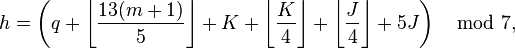
\includegraphics[width=0.8\linewidth,height=0.8\textheight,keepaspectratio=true]{/home/cuvelier/Documents/ESI/Java/2016-2017/DEV1Q2/notes/DEV1Q2/ChallengeBoucle/fr/image/zeller.png}
						\end{center}
                
                    \caption[zeller.png]{zeller.png}
                \end{figure}
                    
            \par
        
      o\`u
      
					\begin{itemize}
				
			\item \verb@h@ est un entier repr\'esentant le jour de la semaine (0 = samedi, 1 = dimanche, 2 = lundi, . . .),
			\item \verb@q@ est un entier repr\'esentant le jour du mois (de 1 \`a 31),
			\item \verb@m@ est un entier repr\'esentant le num\'ero du mois 
				(3 = mars, 4 = avril, . . . Janvier et f\'evrier \'etant consid\'er\'es comme les mois 13 et 14 de l'ann\'ee pr\'ec\'edente. Donc janvier 2016 sera consid\'er\'e comme 13 2015),
			\item \verb@J@ est un entier repr\'esentant year/100 (par exemple 20 pour l'ann\'ee 2016),
			\item \verb@K@ est un entier repr\'esentant l'ann\'ee dans le si\`ecle, c'est \`a dire year mod 100 (par exemple 16 pour l'ann\'ee 2016)
			\item \verb@x/y@ repr\'esente le r\'esultat de \textbf{division enti\`ere} de x par y.
					\end{itemize}
				
      Ainsi, pour le 3 avril 2016, \verb@q@ = 3, \verb@m@ = 3, 
      \verb@J@ = 20 et \verb@K@ = 16. \par
				
      Le r\'esultat \verb@h@ de la congruence de Zeller est ((3+13+16+4+5+100) mod 7) = (141 mod 7) = 1 et donc \textbf{dimanche}.
    
            \par
        
      Une autre r\`egle est n\'ecessaire : celle des ann\'ees bissextiles. \par
				
      En effet, le mois de f\'evrier de ces ann\'ees contient 29 jours au lieu de 28.
      Depuis l'instauration du calendrier gr\'egorien, sont bissextiles les ann\'ees divisibles par 4 mais non divisibles par 100 ou les ann\'ees divisibles par 400. 
      Ainsi, 2016 est une ann\'ee bissextile mais 2015 pas.
    
            \par
        
			
		\subparagraph{Calcul de la cat\'egorie} 
		
					\textcolor{white}{.} \par
				
      \'Ecrivez les algorithmes suivants, dont voici les prototypes :
      
					\begin{itemize}
				
			\item \verb@algorithme isLeapYear(year : entier) → booléen@
            \par
        
          qui re\c coit une ann\'ee au format AAAA et qui renvoie vrai si cette ann\'ee est bissextile et faux si elle ne l'est pas.
        
			\item \verb@algorithme daysInMonth(month, year : entiers) → entier@
            \par
        
          qui retourne le nombre de jours du mois donn\'e en param\`etre.
        
			\item \verb@algorithme isAvailableDate(day, month, year : entiers) → booléen@
            \par
        
          qui re\c coit le jour, le mois et l'ann\'ee d'une date et qui renvoie vrai si cette date est valide et faux si elle ne l'est pas.
          Une date est consid\'er\'ee comme valide si le mois est compris entre 1 et 12 et le jour entre 1 et (le nombre de jours du mois).
        
			\item \verb@algorithme dayOfWeek(day, month, year : entiers) → entier@
            \par
        
          qui retourne un entier correspondant au jour de la semaine (0 = lundi, 1 = mardi, . . .) pour une date donn\'ee en param\`etre. \par
				
          Le param\`etre year est au format AAAA, par exemple 2016.
          Si la date fournie est invalide, l'algorithme lancera une erreur.
            \par
        
			\item \verb@algorithme printDay(day : entier)@
            \par
        
          qui affiche \`a l'\'ecran au format JJ le num\'ero du jour donn\'e en param\`etre.\par
				
          Par exemple, si on donne 1 en param\`etre \`a cette fonction, celle-ci affichera 01.
        
			\item \verb@algorithme printCalendar(month, year : entiers)@
            \par
        
          qui affiche \`a l'\'ecran le calendrier du mois de l'ann\'ee pass\'es en param\`etre, les semaines commen\c cant par le lundi.
        
			\item \verb@algorithme principal@
            \par
        
          qui demande \`a l'utilisateur d'entrer un mois et une ann\'ee au clavier.\par
				
          Si le mois entr\'e n'est pas valide, le programme redemandera la lecture jusqu'\`a obtenir une valeur correcte pour le mois.\par
				
          Ensuite, le programme affichera \`a l'\'ecran le calendrier du mois et de l'ann\'ee lus.
        
					\end{itemize}
				
            \par
        \'Ecrivez le code java correspondant ainsi que la javadoc.
            \par
        
		  Toutes les m\'ethodes sauf la m\'ethode \verb@main@ 
		  seront \'ecrites dans une classe \verb@g12345.boucles.UtilCalendrier@.
    
            \par
        
      La m\'ethode \verb@main@ 
		  sera \'ecrite dans une classe \verb@g12345.boucles.Calendrier@. 
		  Elle attrapera les \'eventuelles exceptions lanc\'ees et affichera alors un message d'erreur explicite.
	\end{abstract}
				\vspace{-2em}\tableofcontents
				\pagestyle{plain}
            \clearpage
            \fancyhead[L,C,R]{}
            \fancyfoot[L,C]{}
            \fancyfoot[R]{ \scriptsize{\textcolor{gray}{
				ChallengeBoucle - page \thepage}}}
				\thispagestyle{fancy}
				\pagestyle{fancy}
	   
            
				\end{document}
			